\documentclass[10pt,usepdftitle=false]{beamer}

\usepackage[american]{babel}
\usepackage[utf8]{inputenc}
%\usepackage{soul}
\usepackage{amsmath}
\usepackage{amssymb}
\usepackage{textcomp}
\usepackage{listings}
\lstset{
  language=haskell,
  upquote=true,
  basicstyle=\ttfamily,          % print whole listing in typewriter
  keywordstyle=\color{blue}\bfseries, % bold blue keywords
  %identifierstyle=,           % nothing happens
  commentstyle=\color{green}, % green comments
  stringstyle=\color{red},      % typewriter type for strings
  showstringspaces=false     % no special string spaces
}
\usepackage[all]{xy}
\usepackage{tikz}
%\usetikzlibrary{arrows,shapes,automata}
\usepackage{graphicx}
\usepackage[bibstyle=beamer,citestyle=authoryear-comp,doi=false,isbn=false,eprint=false,maxnames=10]{biblatex}
\bibliography{../defeo}
\usepackage{../mysymbols}
\usepackage{array}

\mode<presentation>{%
  \usetheme{these}
}

\title[Fast Algorithms for Towers of Finite Fields and Isogenies]{
  \def\svgwidth{2.63ex}
  \def\exclfont{\scriptsize\rmfamily}
  %% Creator: Inkscape inkscape 0.48.0, www.inkscape.org
%% PDF/EPS/PS + LaTeX output extension by Johan Engelen, 2010
%% Accompanies image file 'bigescargot-color.pdf' (pdf, eps, ps)
%%
%% To include the image in your LaTeX document, write
%%   \input{<filename>.pdf_tex}
%%  instead of
%%   \includegraphics{<filename>.pdf}
%% To scale the image, write
%%   \def\svgwidth{<desired width>}
%%   \input{<filename>.pdf_tex}
%%  instead of
%%   \includegraphics[width=<desired width>]{<filename>.pdf}
%%
%% Images with a different path to the parent latex file can
%% be accessed with the `import' package (which may need to be
%% installed) using
%%   \usepackage{import}
%% in the preamble, and then including the image with
%%   \import{<path to file>}{<filename>.pdf_tex}
%% Alternatively, one can specify
%%   \graphicspath{{<path to file>/}}
%% 
%% For more information, please see info/svg-inkscape on CTAN:
%%   http://tug.ctan.org/tex-archive/info/svg-inkscape

\begingroup
  \makeatletter
  \providecommand\color[2][]{%
    \errmessage{(Inkscape) Color is used for the text in Inkscape, but the package 'color.sty' is not loaded}
    \renewcommand\color[2][]{}%
  }
  \providecommand\transparent[1]{%
    \errmessage{(Inkscape) Transparency is used (non-zero) for the text in Inkscape, but the package 'transparent.sty' is not loaded}
    \renewcommand\transparent[1]{}%
  }
  \providecommand\rotatebox[2]{#2}
  \ifx\svgwidth\undefined
    \setlength{\unitlength}{153.08584512pt}
  \else
    \setlength{\unitlength}{\svgwidth}
  \fi
  \global\let\svgwidth\undefined
  \makeatother
  \begin{picture}(1,0.63533296)%
    \put(0,0){\includegraphics[width=\unitlength]{\artdir/bigescargot\suffix.pdf}}%
    \put(0.94506612,0.46275528){\color[rgb]{0,0,0}\makebox(0,0)[lb]{\smash{\exclfont\textbf{!}}}}%
  \end{picture}%
\endgroup
~~~Fast Algorithms\\
  \normalsize\textcolor{black}{for Towers of Finite Fields\\and Isogenies}}
\hypersetup{pdftitle={Fast Algorithms for Towers of Finite Fields and Isogenies},pdfauthor={Luca De Feo}}
\author{Luca~De~Feo}
\institute[LIX \& INRIA Saclay]{LIX, École Polytechnique \& INRIA Saclay, Projet TANC}
\date[December 13, 2010]{December 13, 2010\\École Polytechnique, Palaiseau}


\AtBeginSection[]
{
  \begin{frame}<beamer>
    \frametitle{Outline}
    \tableofcontents[currentsection]
  \end{frame}
}


\begin{document}

{\setbeamertemplate{footline}[these theme title]
\begin{frame}
  \titlepage
\end{frame}
}

%%
%%

\section{Introduction}

\begin{frame}
  \frametitle{The Discrete Logarithm Problem}
  
  \begin{columns}
    \begin{column}{0.4\textwidth}
      \begin{tikzpicture}
        \begin{scope}
          \foreach \alpha in {0,...,4} {
            \filldraw (-65-25*\alpha:2) circle (2pt);
          }
          \foreach \alpha in {0,...,3} {
            \draw[->] (-65-25*\alpha:2) arc (-65-25*\alpha:-85-25*\alpha:2);
            \draw (-90-25*\alpha:2.3) node {$g^\alpha$};
          }
          \draw (-65:2.3) node {$g^{n-1}$};
          \draw[densely dotted,gray] (-65:2) arc (-65:195:2);
          \draw (0,0) node {\Large $G=\langle g\rangle$};
        \end{scope}
        
        \begin{uncoverenv}<2->
          \begin{scope}[yshift=-3cm]
            \foreach \alpha in {0,...,4} {
              \filldraw (-65-25*\alpha:2) circle (2pt);
            }
            \foreach \alpha in {0,...,3} {
              \draw[->] (-65-25*\alpha:2) arc (-65-25*\alpha:-85-25*\alpha:2);
              \draw (-90-25*\alpha:2.3) node {$\alpha$};
            }
            \draw (-65:2.3) node {$n-1$};
            \draw[densely dotted,gray] (-65:2) arc (-65:48:2);
            \draw[densely dotted,gray] (132:2) arc (132:195:2);
            \draw (0,-0.5) node {\Large $\Z/n\Z$};
          \end{scope}
        \end{uncoverenv}
        
        \begin{uncoverenv}<3->
          \foreach \alpha in {0,...,4}
          \usebeamercolor[fg]{alerted text}
          \draw[dashed] (-65-25*\alpha:2) -- ++(0,-3cm);
        \end{uncoverenv}
      \end{tikzpicture}
    \end{column}
    \begin{column}{0.6\textwidth}
      \begin{block}{Exponentiation in a cyclic group}
        Let $G=\langle g\rangle$ be a cyclic group of order $n$.
        Define
        \begin{align*}
          \exp_g : \Z/n\Z &\ra G\text{,}\\
          x&\mapsto g^x\text{.}
        \end{align*}
      \end{block}

      \begin{block}<2->{Discrete logarithm} $\exp_g$ is an
        isomorphism. Its inverse is called \emph{discrete logarithm}.
        \begin{align*}
          \log_g : G &\ra \Z/n\Z\text{,}\\
          g^x&\mapsto x\text{.}
        \end{align*}

        \begin{uncoverenv}<3-> Computing it is called the
          \alert{Discrete Logarithm Problem} (DLP) of $G$.
        \end{uncoverenv}
      \end{block}
    \end{column}
  \end{columns}
\end{frame}

%%

\begin{frame}
  \frametitle{Elliptic curve cryptography}

  \vspace{-1mm}

  \begin{columns}
    \begin{column}{0.4\textwidth}
      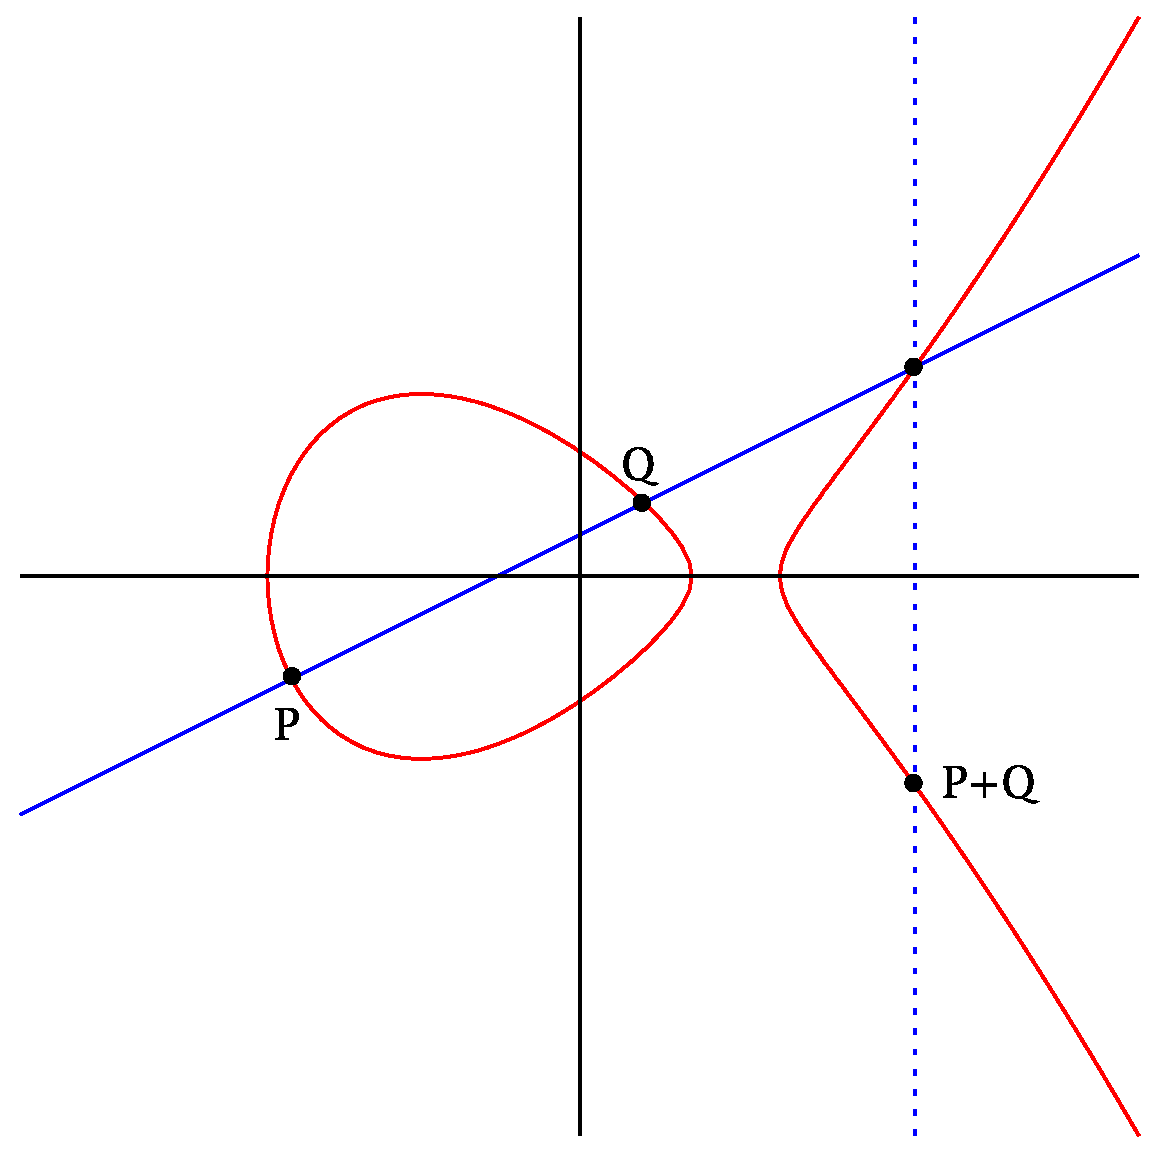
\includegraphics[width=\textwidth]{../isogeny/ec-add.pdf}
    \end{column}
    \begin{column}{0.55\textwidth}
      \begin{block}{Elliptic curve (Weierstrass form)}
        \[E : y^2 = x^3 + ax + b\text{;}\]
      
        The set of points of an elliptic curve is endowed with a group
        law via the chord-and-tangent law.
      \end{block}
    
      \begin{block}{}
        \emph{Hasse bound:} $\card{E(\F_q)} \sim q$.
      \end{block}
    \end{column}
  \end{columns}

  \begin{center}
    \begin{tabular}{l | l | l}
      &\emph{\textbf{Finite field crypto}} & \emph{\textbf{Elliptic curve crypto}}\\
      \hline
      \emph{Group} & $\F_q^\ast$ & $E(\F_q)$\\
      \emph{Protocols} & El Gamal, DSA, \dots & ECDH, ECDSA, ECMQV, \dots\\
      \emph{Key sizes}\footnote{\url{http://csrc.nist.gov/publications/nistpubs/800-57/sp800-57-Part1-revised2_Mar08-2007.pdf}}  & 1024, 2048, 3072 & 160, 225, 256 \\
    \end{tabular}
  \end{center}

\end{frame}

%%

\begin{frame}
  \frametitle{Multiplication}
  
\end{frame}

%%

\begin{frame}
  \frametitle{Isogenies between elliptic curves}
  
  \vspace{-2mm}

  {\large \[\I:E\to E'\]} 
  \emph{\textbf{(Separable) isogeny:}} (separable)
  non-constant rational morphism preserving the identity.
  
  \begin{block}{Properties}
    \begin{itemize}
    \item Isogeny = rational map $\;+\;$ group morphism;
    \item Finite kernel, surjective (in $\clot{\K}$);
    \end{itemize}
  \end{block}

  \vspace{-1mm}

  \begin{block}{
	\begin{overprint}
	\onslide<1> Multiplication	
	\onslide<2> Frobenius endomorphism
	\onslide<3> Separable isogeny, odd degree (simplified Weierstrass model)
	\end{overprint}
      }
    \begin{overprint}
      \onslide<1>
      \[\begin{aligned}
	{}[m] : E(\clot{\K}) &\rightarrow E(\clot{\K})\\
	                   P &\mapsto [m]P
      \end{aligned}\]
      $\ker\I = E[m]$.

      \onslide<2>
      \[\begin{aligned}
	\frob : E(\clot{\K}) &\rightarrow E(\clot{\K})\\
	               (X,Y) &\mapsto (X^q,Y^q)
      \end{aligned}\]
      $\ker\frob = \{\0\}$.

      \onslide<3>
      \[\quad\I(X,Y) = \left(\frac{g(X)}{h^2(X)},
      cY\left(\frac{g(X)}{h^2(X)}\right)'\right)\]
      $\card{\ker\I} \;=\; 2\deg h + 1\;$ odd.
    \end{overprint}
  \end{block}  
\end{frame}

%%

\begin{frame}
  \frametitle{Why compute (large) isogenies over finite fields?}
  
  \begin{block}{SEA algorithm (\cite{schoof85,elkies92,atkin88})}
    \begin{description}
    \item[Hasse bound] \hfill{\large\emph{$\card{E(\F_q)}= q-t+1$}};\hfill\strut
    \item[Schoof] Compute $t$ modulo small primes
      $\ell\;\Leftrightarrow$ compute the action of $\frob_q$ on
      \emph{$E[\ell]\isom(\Z/\ell\Z)^2$};
    \item[Atkin] Determine the order of the roots of $X^2 -tX +q$ by
      factoring the $\ell$-th modular polynomial.
    \item[Elkies] Compute an $\ell$-isogeny $\I$ and the action of
      $\frob_q$ on \emph{$\ker\I\isom\Z/\ell\Z\subset E[\ell]$};
    \end{description}
  \end{block}

  \begin{block}{Other cryptographic applications}
    \begin{itemize}
    \item Tranfer DLPs between curves (\cite{gaudry+hess+smart02,smith09});
    \item Construct new cryptosystems (\cite{teske06,rostovtsev+stolbunov06});
    \item Construct hash functions (\cite{charles+lauter+goren09});
    \item Compute modular polynomials (\cite{sutherland10:modpol});
    \item Compute the endomorphism ring (\cite{kohel,sutherland10:hilbert}).
    \end{itemize}
  \end{block}
\end{frame}

%%
%%

\section{Computing isogenies over finite fields}

\begin{frame}
  \frametitle{Vélu's formulas}
  
  \begin{block}{Compute an isogeny with given kernel (\cite{velu71})}
    Given the kernel $H$, computes $\;\I : E\to E/H\;$ given by
    \begin{align*}
      &\I(\0_E) = \I(\0_{E/H})\text{,}\\
      &\begin{aligned}
        \I(P) = \Biggl(x(P) + \sum_{Q\in H^\ast}x(P+Q) - x(Q),
        y(P) + \sum_{Q\in H^\ast}y(P+Q) - y(Q) \Biggr) \text{.}
      \end{aligned}
    \end{align*}
  \end{block}

  \begin{block}{In practice, given $h(x)$ vanishing on $H$}
    {\footnotesize
      \[
      y^2 = f(x)
      \qquad
      t = \sum_{Q\in H^\ast} f'(Q)\text{,}
      \quad
      u = \sum_{Q\in H^\ast} 2f(Q)\text{,}
      \quad
      w = u + \sum_{Q\in H^\ast} x(Q)f'(Q)\text{,}\]}
    \[\alert{\I(x,y) = \left(\frac{g(x)}{h(x)}, y\left(\frac{g(x)}{h(x)}\right)'\right)}
    \quad\text{with}\quad
    \frac{g(x)}{h(x)} = x + t\frac{h'(x)}{h(x)} - u\left(\frac{h'(x)}{h(x)}\right)'\]
  \end{block}
\end{frame}

%%

\begin{frame}
  \frametitle{Isogeny computation}
  
  \begin{center}
    \large
    Given $E, E', \ell$, compute $\I:E\to E'$
  \end{center}

  By Vélu's formulas:
  $\I(x,y) = \left(\frac{g(x)}{h(x)}, y\left(\frac{g(x)}{h(x)}\right)'\right)$,
  hence
  \[(x^3 + ax + b){\left(\frac{g(x)}{h(x)}\right)'}^2 =
  \left(\frac{g(x)}{h(x)}\right)^3 + a'\frac{g(x)}{h(x)} + b'\]
  
  \begin{block}{BMSS algorithm \parencite{bostan+morain+salvy+schost08}}
    Power series solution 
  \end{block}

  \begin{block}{Lercier $p=2$}
    
  \end{block}

  \begin{block}{\cite{lercier+sirvent08}}
    When $p$ exceeds the precision, a division by zero happens:
    \begin{itemize}
    \item Lift $E$ and $E'$ in the $p$-adics while keeping $\Phi_\ell\left(j(\tilde{E}),j(\tilde{E}')\right)=0$;
    \item Apply BMSS in $\Q_q$.
    \end{itemize}
  \end{block}
\end{frame}

%%

\begin{frame}
  \frametitle{Couveignes' algorithm (\cite{couveignes96})}
  
  \begin{center}
    \large
    Given $E, E', \ell$, compute $\I:E\to E'$
  \end{center}

  \begin{center}
    \emph{\textbf{Idea:}} Send $E[p^k]$ over $E'[p^k]$
  \end{center}
  
  \begin{itemize}
  \item \alert<4>{Compute the extensions $\U_i/\F_q$
    such that $E[p^i]$ is defined in $\U_i$;}
    \hfill\emph{\temporal<2>{}{$\tildO(\ell^2)$}{\alert{$\tildO(\Mult(\ell))$}}}
  \item Pick $\;k\;$ \emph{large enough} ($k\sim\log_p4\ell$);
  \item \alert<4>{Compute $\;P$, a generator of $\;E[p^k]$;}
    \hfill\emph{\temporal<2>{}{$\tildO(\ell^2)$}{\alert{$\tildO(\Mult(\ell))$}}}
  \item \alert<4>{Compute $\;P'$, a generator of $\;E'[p^k]$;}
    \hfill\emph{\temporal<2>{}{$\tildO(\ell^2)$}{\alert{$\tildO(\Mult(\ell))$}}}
  \item Compute the polynomial $\;T\;$ vanishing $\;E[p^k]$;
    \hfill\emph{\temporal<2>{}{$\tildO(\ell^2)$}{\alert<3>{$\tildO(\Mult(\ell))$}}}
  \item For $j\in\left(\Z/p^k\Z\right)^\ast$
    \begin{itemize}
      \normalsize
    \item Interpolate $\;A : x(P) \mapsto x([j]P')$;
      \hfill\emph{\temporal<2>{}{$\tildO(\ell^2)$}{\alert<3>{$\tildO(\Mult(\ell))$}}}
    \item Reconstruct a rational fraction  $\;\frac{g}{h}\equiv A \bmod T$;
      \hfill\emph{\alt<1>{}{$\tildO(\Mult(\ell))$}}
    \end{itemize}
    Stop when $\frac{g}{h}$ is an isogeny.
    \hfill\emph{\alt<1>{}{$\ell$ times on average}}
  \end{itemize}
\end{frame}

%%

\begin{frame}
  \frametitle{Couveignes' algorithm (\cite{couveignes96})}
  
  \begin{center}
    \large
    Given $E, E', \ell$, compute $\I:E\to E'$
  \end{center}

  \begin{center}
    \emph{\textbf{Idea:}} Send $E[p^k]$ over $E'[p^k]$
  \end{center}
  
  \begin{itemize}
  \item Compute the extensions $\U_i/\F_q$ such that $E[p^i]$ is
    defined in $\U_i$;
  \item Pick $\;k\;$ \emph{large enough} ($k\sim\log_p4\ell$);
  \item Compute $\;P$, a generator of $\;E[p^k]$;
  \item Compute $\;P'$, a generator of $\;E'[p^k]$;
  \item Compute the polynomial $\;T\;$ vanishing $\;E[p^k]$;
  \item Interpolate $\;A : x(P) \mapsto x(P')$;
  \item Reconstruct a rational fraction  $\;\frac{g}{h}\equiv A \bmod T$;
  \item \alert{If $\frac{g}{h}$ is an isogeny}, done; otherwise pick another $P'$.
  \end{itemize}
\end{frame}

%%

\begin{frame}
  \frametitle{How to recognize an isogeny?}

  \begin{itemize}
    \setlength{\itemsep}{\baselineskip}
  \item \emph{\textbf{Degree:}} $\frac{g}{h}\;$ with $\;\deg g=\ell$, $\;\deg h = \ell-1$;\hfill\alert{$O(1)$}
  \item \emph{\textbf{Square factor:}} $h = \prod_{Q\in H^\ast}(X-
    x(Q)) = f^2\;$ if $\ell$ odd;\hfill\emph{$\tildO(\Mult(\ell))$}
  \item \emph{\textbf{Group action:}} Test with random points;\hfill\emph{$O(\ell)$}
  \item \emph{\textbf{Factor of the $\ell$-division polynomial:}}
    Compute $\phi_\ell\bmod h$.\hfill\emph{$\tildO(\Mult(\ell))$}
  \end{itemize}
\end{frame}

%%

\begin{frame}
  \frametitle{How to recognize an isogeny?}
  
  \[AU_i + TV_i = R_i  \qquad\Leftrightarrow\qquad  A\equiv \frac{R_i}{U_i} \bmod T\]
  \[\ell = 11\]
  \pause
  \begin{center}
  \begin{tabular}{c | c}
    $\deg R_i$ & $\deg U_i$ \\
    $3141592653589793238462643$ & 0 \\
    \pause
    $3141592653589793238462642$ & 1 \\
    \pause
    $3141592653589793238462641$ & $2$ \\
    \pause
    \vdots & \vdots\\
    $3141592653589793238462634$ & $9$ \\
    \pause\pause
    \Huge\alert{$11$} & \Huge\alert{$10$}\\
    \pause
    $10$ & $3141592653589793238462633$\\
    \vdots & \vdots
  \end{tabular}
  \end{center}
\end{frame}

%%

\begin{frame}
  \frametitle{Isogenies of unknown degree}
  
  \begin{itemize}
  \item This pattern is extremely rare.
  \item This is the only phase of Couveignes' algorithm that depends on $\ell$.
  \end{itemize}

  \begin{itemize}
  \item<2-> \large Actually, this does not really depend on $\ell$,
    just on the existence of a \emph{gap}.
  \item<2-> \large If $\ell$ is not known in advance, it is enough to
    look for a \emph{gap}.
  \item<2-> \large Thus, any isogeny of degree $\ll p^k$ can be
    computed with one single run of Couveignes' algorithm.
  \end{itemize}  
\end{frame}

%%

\begin{frame}
  \frametitle{Comparison of isogeny algorithms}
  
  \begin{figure}
    \centering
    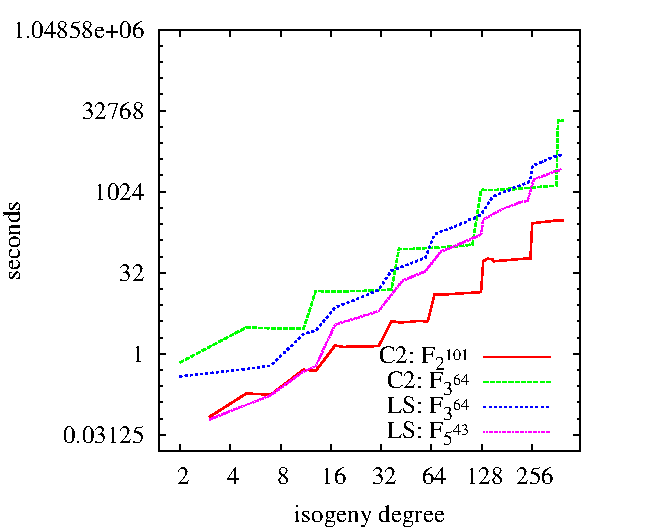
\includegraphics[height=0.5\textwidth]{../isogeny/C2-LS}
    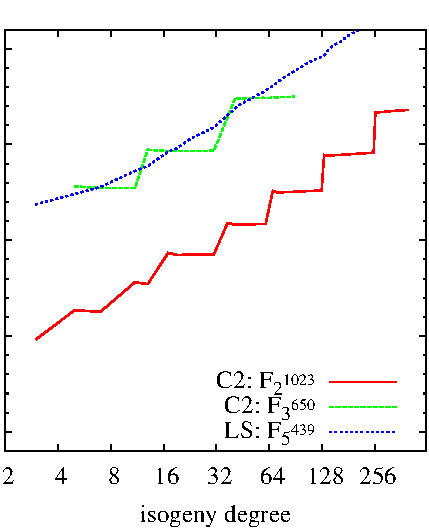
\includegraphics[height=0.5\textwidth]{../isogeny/C2-LS2}
    \caption{Comparative timings for \cite{couveignes96} (C2) and
      \cite{lercier+sirvent08} (LS) over various curves. Plot in
      logarithmic scale.}
  \label{fig:comp}
\end{figure}
\end{frame}

%%
%%

\section{Artin-Schreier towers}

\begin{frame}<1-2>
  \frametitle{The field of definition of $E[p^k]$}
  
  \begin{columns}
    \begin{column}{0.3\textwidth}
      \begin{overlayarea}{\textwidth}{0.9\textheight}
        \begin{onlyenv}<1>
          \large\[\xymatrix@C=20pt{
            *[r]{\U_k} \ar@{-}[d]^p & E[p^k] \ar@{-->}[l]\\
            *[r]{\U_{k-1}} \ar@{--}[dd] & E[p^{k-1}] \ar@{-->}[l]\\
            \\
            *[r]{\U_2} \ar@{-}[d]^p & E[p^2] \ar@{-->}[l]\\
            *[r]{\U_1} \ar@{-}[d] & E[p] \ar@{-->}[l]\\
            *[r]{\F_q}
          }\]
        \end{onlyenv}
        \begin{onlyenv}<2>
          \Large\[\xymatrix{
            *+[r]{\U_k = \frac{\U_{k-1}[X_k]}{P_{k-1}(X_k)}}\ar@{-}[d]^p\\
            *+[r]{\U_{k-1}} \ar@{--}[dd]\\
            \\
            *+[r]{\U_{1} = \frac{\U_0[X_1]}{P_0(X_1)}} \ar@{-}[d]^p\\
            *+[r]{\U_{0} = \F_q = \frac{\F_p[X_0]}{Q(X_0)}}
          }\]
        \end{onlyenv}
      \end{overlayarea}
    \end{column}
    \begin{column}{0.65\textwidth}
      \begin{block}{$p$-descent (\cite{voloch90})}
        If $\;P_i=(x_i,y_i)\;$ generates $\;E[p^i]$, the solution to
        \[X^p - X = \frac{\sqrt[p]{y_i\beta_E(x_i)}}{\sqrt[p-1]{H_E}}\]
        generates $\;E[p^{i+1}]$. $y_i=?$
      \end{block}

      \begin{block}<2>{Artin-Schreier Towers over finite fields}
        $\LK/\K$ extension: Artin-Schreier polynomial:
        
        \begin{center}
          \Large\emph{$X^p - X - \alpha$}
        \end{center}

        \alert{ANY} separable extension of degree $p$ can be expressed
        this way.
      \end{block}
    \end{column}
  \end{columns}
\end{frame}

%%

\begin{frame}
  \frametitle{Slow towers}
  
\end{frame}

%%

\begin{frame}
  \frametitle{One fast tower, many fast towers! (\cite{couveignes00})}
  
  Theorem (Couveignes): Be fast!
  
  \begin{center}
    Fast tower

    \bigskip

    \Large$\xymatrix{
      \only<3>{E[p^k]\ar@{-->}[r]} & \only<2->{\U_k \ar@{-}[d]\ar[r]}      & \LK_k \ar@{-}[d]      & \only<2->{\U_k' \ar@{-}[d]\ar[l]}& \only<3>{E[p^k]\ar@{-->}[l]}\\
      &\only<2->{\U_{k-1} \ar@{--}[dd]\ar[r]} & \LK_{k-1} \ar@{--}[dd] & \only<2->{\U_{k-1}' \ar@{--}[dd]\ar[l]}\\
      \\
      &\only<2->{\U_1 \ar@{-}[dr]\ar[r]}     & \LK_1 \ar@{-}[d]      & \only<2->{\U_1' \ar@{-}[dl]\ar[l]}\\
      &                    &\LK_0
    }$
  \end{center}
\end{frame}

%%

\begin{frame}
  \frametitle{A fast tower}

\end{frame}

%% 

\begin{frame}
  \frametitle{A fast tower}

  \vspace{-2mm}

  \begin{columns}
    \begin{column}{0.3\textwidth}
      \Large\[\xymatrix{
        *+[r]{\LK_k = \frac{\U_{k-1}[X_k]}{P_{k-1}(X_k)}}\ar@{-}[d]^p\\
        *+[r]{\LK_{k-1}} \ar@{--}[d]\\
        *+[r]{\LK_1 = \frac{\U_0[X_1]}{P_0(X_1)}} \ar@{-}[d]^p\\
        *+[r]{\LK_0 = \F_q = \frac{\F_p[X_0]}{Q(X_0)}}
      }\]
    \end{column}
    \begin{column}{0.65\textwidth}
      \begin{block}{Our construction}
        Let $\;x_0 = X_0\;$ such that
        $\;\Tr_{\LK_0/\F_p}(x_0) \ne 0$, let
        \begin{align*}
          P_0 \quad&=\quad X^p - X - x_0\\
          P_i \quad&=\quad X^p - X - x_i^{2p-1}
        \end{align*}
        with $\;x_{i+1}\;$ a root of $\;P_i\;$ in $\;\LK_{i+1}$.

        \alert{This tower is such that $x_i$ generates $\LK_i/\F_p$.} Howzat?
      \end{block}

      \begin{block}{Two ways to represent $\LK_k$}
        \begin{itemize}
        \item Univariate basis: $\;\LK_k=\F_p[Z]/Q_k(Z)$;
        \item Multivariate basis: $\;\LK_k=\F_p[X_0,X_1,\ldots,X_k]/(Q,P_0,\ldots,P_{k-1})$.
        \end{itemize}
        \alert{A fast change of basis is the key to fast arithmetic:}
        \begin{itemize}
        \item Multiplication is faster in \emph{univariate};
        \item Embeddings are faster in \emph{multivariate}.
        \end{itemize}
      \end{block}
    \end{column}
  \end{columns}
\end{frame}

%%

\begin{frame}
  \frametitle{Fast tower example}
  
\end{frame}

%%

\begin{frame}
  \frametitle{Change of basis}

  \begin{block}{Univariate $\ra$ multivariate}
    Recursive algorithm: given $\;a(Z)\in\F_p[Z]/Q_k(Z)$
    \begin{itemize}
    \item Split $a$ in $p$ parts;
    \item convert recursively to multivariate;
    \item recombine using Horner's rule.
    \end{itemize}
    Simple and fast: \emph{$\;O(\Mult(\ell) + \ell\log^2\ell)$}!
  \end{block}

  \begin{block}{Multivariate $\ra$ univariate}
    By \textit{trace formulas} (\cite{rouiller99}):
      \[
      a(Z) = \frac{A(Z)}{Q_k'(Z)}
      \qquad\text{where}\qquad
      A(T) = Q_k(T)\alert<2>{\sum_{i\ge 0}\frac{\Tr aZ^i}{T^{i+1}}}
      \text{.}\]
    \begin{itemize}
    \item Compute the \textit{trace form} $\;\Tr\;$ and the form
      $\;a\cdot\Tr : x\mapsto \Tr ax$;
    \item \alert<2>{compute $\;\sum_{i\ge 0}\frac{\Tr aZ^i}{T^{i+1}}$}, deduce $\;a(Z)$.
    \end{itemize}
  \end{block}
\end{frame}

%%

\begin{frame}
  \frametitle{Duality (\cite{shoup95,shoup99,bostan+salvy+schost03})}

  \vspace{-6mm}

  \begin{columns}[b]
    \begin{column}{0.5\textwidth}
      \begin{center}
        \textbf{Polynomial evaluation}$:k[T]\ra\K/k$
        \[g\mapsto g(\sigma)\]
      \end{center}
    \end{column}
    \begin{column}{0.5\textwidth}
      \begin{center}
        \textbf{Power projection}$:(\K/k)^\ast\ra k[T]^\ast$
        \[\ell \mapsto \sum_{i>0} \frac{\ell(\sigma^i)}{T^i}\]
      \end{center}
    \end{column}
  \end{columns}

  \begin{block}{Univariate $\ra$ multivariate $=$ Polynomial evaluation}
    If $Z \mapsto \zeta\;$ (with $\zeta\in\U_k$ written on the
    multivariate basis):
    \[a(Z) = a_dZ^d + \cdots + a_1Z + a_0 \quad\mapsto\quad a_d\zeta^d + \cdots + a_1\zeta + a_0 =a(\zeta)\text{.}\]
  \end{block}

  \begin{block}{$($Univariate $\ra$ bivariate$)^\ast=$ Power projection}
    \begin{align*}
      \Tr &\quad\mapsto\quad \sum_{i\ge0}\frac{\Tr\zeta^i}{T^i}\text{,}\\
      a\cdot\Tr &\quad\mapsto\quad \sum_{i\ge0}\frac{\Tr a\zeta^i}{T^i}\text{.}
    \end{align*}
  \end{block}
\end{frame}

%%
%%

\section{The transposition principle}

\begin{frame}
  \frametitle{The transposition principle}

  \begin{quote}
    \large ``Let $\pspace$ be an arbitrary set. To any $R$-algebraic
    algorithm $A$ computing a family of linear functions $(f_p:M\ra
    N)_{p\in\pspace}$ corresponds an $R$-algebraic algorithm
    $\dual{A}$ computing the \emph{dual family}
    $(\dual{f}_p:\dual{N}\ra\dual{M})_{p\in\pspace}$. The algebraic
    time and space complexities of $\dual{A}$ are bounded by the time
    complexity of $A$.''
  \end{quote}
  
\end{frame}

%%

\begin{frame}
  \frametitle{Transposition of arithmetic circuits}

  Plus dynamique !!

  \begin{columns}
    \begin{column}{0.6\textwidth}
      \begin{center}
        Arithmetic circuits are like diagrams enriched with a
        \emph{product}. In particular they can be \emph{transposed}:
      \end{center}

      \begin{center}
      \begin{tikzpicture}
        \tikzstyle{node}=[circle,thick,draw=black,minimum size=4mm]
        \tikzstyle{arg}=[rectangle,thin,draw=black,minimum size=4mm]
        
        \begin{scope}
          \node[arg](in1){$x_1$};
          \node[arg,right of=in1](in2){$x_2$};
          \node[arg,right of=in2](in3){$x_3$};
          
          \node[node,below of=in1](plus1){$+$};
          \node[node,right of=plus1](H){$\hub$};

          \node[node,below of=plus1](plus2){$+$};
          \node[node,right of=plus2](times){$\rmul{2}$};

          \node[arg,below of=plus2,xshift=6mm](out1){$y_1$};
          \node[arg,right of=out1](out2){$y_2$};

          \path[->]
          (in1) edge (plus1)
          (in2) edge (H)
          (in3) edge (out2)
          (H) edge (plus1)
          (H) edge (times)
          (plus1) edge (plus2)
          (times) edge (plus2)
          (plus2) edge (out1);
        \end{scope}

        \begin{uncoverenv}<2->
        \begin{scope}[xshift=3cm, yshift=-0.17\textheight]
          \node(x){\Huge $\leftrightarrow$};
        \end{scope}

        \begin{scope}[xshift=4.2cm]
          \node[arg](in1){$\dual{x_1}$};
          \node[arg,right of=in1](in2){$\dual{x_2}$};
          \node[arg,right of=in2](in3){$\dual{x_3}$};
      
          \node[node,below of=in1](plus1){\alt<3>{$\hub$}{$+$}};
          \node[node,right of=plus1](H){\alt<3>{$+$}{$\hub$}};
          
          \node[node,below of=plus1](plus2){\alt<3>{$\hub$}{$+$}};
          \node[node,right of=plus2](times){$\rmul{2}$};
          
          \node[arg,below of=plus2,xshift=6mm](out1){$\dual{y_1}$};
          \node[arg,right of=out1](out2){$\dual{y_2}$};
          
          \path[<-]
          (in1) edge (plus1)
          (in2) edge (H)
          (in3) edge (out2)
          (H) edge (plus1)
          (H) edge (times) 
          (plus1) edge (plus2)
          (times) edge (plus2)
          (plus2) edge (out1);
        \end{scope}
        \end{uncoverenv}
      \end{tikzpicture}
      \end{center}

      \begin{center}
        \uncover<3>{This can be made precise using category theory.}
      \end{center}
    \end{column}
    \begin{column}{0.4\textwidth}
      \begin{align*}
        y_1 &= x_1 + 3x_2\\
        y_2 &= x_3
      \end{align*}
      
      \Large
      \begin{gather*}
        \begin{pmatrix}
          1 & 3 & 0\\
          0 & 0 & 1
        \end{pmatrix}\\
        \uncover<2->{\updownarrow}\\
        \uncover<2->{\begin{pmatrix}
          1 & 0\\
          3 & 0\\
          0 & 1\\
        \end{pmatrix}}
      \end{gather*}
    \end{column}
  \end{columns}
\end{frame}

%%

\begin{frame}
  \frametitle{\emph{Automatic} transposition?}

  \begin{itemize}
  \item Algorithms are hard to transpose, transposed algorithms are
    hard or impossible to understand;
  \item How to be confident that a transposed algorithm is well
    implemented if no one understands it?
  \item When proving programs with a proof assistant, why should we do
    the work twice?
  \end{itemize}

  \begin{block}{Previous work}
    \begin{itemize}
    \item Originally discovered in \emph{electrical network theory} by
      \cite{bordewijk57} (only works for $\C$); some authors attribute
      the discovery to Tellegen, Bordewijk's director, but this is
      debated;
    \item \cite{fiduccia:phd} and \cite{hopcroft+musinski73}:
      transposition of \emph{bilinear chains}, the most complete
      formulation (non-commutative rings);
    \item Special case of \emph{automatic differentiation}
      \cite{baur+strassen83};
    \item In \emph{computer algebra}, popularized by Shoup, von zur
      Gathen, Kaltofen,\dots
    \item \cite{bostan+lecerf+schost:tellegen} improve algorithms for
      polynomial evaluation and solve an open question on space
      complexity.
    \end{itemize}
  \end{block}
\end{frame}

%%

% \begin{frame}
%   \frametitle{Multilinearity}

%   \begin{center}
%     \large
%     Does it make sense to transpose $\;c:=a*b$?
%   \end{center}

%   \begin{center}
%     \begin{tikzpicture}
%       \tikzstyle{node}=[circle,thick,draw=black,minimum size=4mm]
%       \tikzstyle{arg}=[rectangle,thin,draw=black,minimum size=4mm]
%       \tikzstyle{nodeg}=[circle,thick,draw=gray,minimum size=4mm]
%       \tikzstyle{argg}=[rectangle,thin,draw=gray,minimum size=4mm]
      
%       \begin{scope}
%         \node[arg](in1){$x_1$};
%         \node[arg,right of=in1](in2){$x_2$};
%         \node[arg,right of=in2](in3){$x_3$};
%         \node[node,below of=in1,xshift=5mm](times1){$*$};
%         \node[node,below of=times1,xshift=5mm](times2){$*$};
%         \node[arg,below of=times2](out){$y_1$};
        
%         \path[->]
%         (in1) edge (times1)
%         (in2) edge (times1)
%         (times1) edge (times2)
%         (in3) edge (times2)
%         (times2) edge (out);
%       \end{scope}
      
%       \begin{scope}[xshift=4cm]
%         \node[argg](in1){\color{gray}{$x_1$}};
%         \node[arg,right of=in1](in2){$x_2$};
%         \node[argg,right of=in2](in3){\color{gray}{$x_3$}};
%         \node[node,below of=in1,xshift=5mm](times1){$*_{x_1}$};
%         \node[node,below of=times1,xshift=5mm](times2){$*_{x_3}$};
%         \node[arg,below of=times2](out){$y_1$};
        
%         \path[->]
%         (in2) edge (times1)
%         (times1) edge (times2)
%         (times2) edge (out);
        
%         \path[->,draw=gray,dashed]
%         (in1) edge (times1)
%         (in3) edge (times2);
%       \end{scope}
      
%       \begin{scope}[xshift=8cm]
%         \node[arg](in1){$x_3$};
%         \node[arg,right of=in1](in2){$y_1^\ast$};
%         \node[arg,right of=in2](in3){$x_1$};
%         \node[node,below of=in1,xshift=5mm](times1){$*$};
%         \node[node,below of=times1,xshift=5mm](times2){$*$};
%         \node[arg,below of=times2](out){$x_2^\ast$};

%         \path[->]
%         (in2) edge (times1)
%         (times1) edge (times2)
%         (times2) edge (out)
%         (in3) edge (times2)
%         (in1) edge (times1);
%       \end{scope}
%     \end{tikzpicture}  
%   \end{center}

%   \begin{itemize}
%   \item Most applications require to \emph{linearize} a multi-linear
%     program.
%   \item Can we automatically deduce any possible linearisation of a
%     program?
%   \item \alert{Type inference systems can help us}
%   \end{itemize}
% \end{frame}

% %%

% \begin{frame}[fragile]
%   \frametitle{Linearity inference}

%   \begin{center}
%     Suppose given a type \lstinline{R} implementing a ring. We want to
%     define types \alert{\lstinline{L}} (for \emph{linear}) and
%     \alert{\lstinline{S}} (for \emph{scalar}) such that the following
%       equations hold
%   \end{center}
  
%   \begin{columns}
%     \begin{column}{0.5\textwidth}
%   \begin{semiverbatim}
%     plus :: L -> L -> L
%     plus :: S -> S -> S
%   \end{semiverbatim}
%     \end{column}
%     \begin{column}{0.5\textwidth}
%       \uncover<2>{\[\forall
%         \alpha\in\{L,S\}.\alpha\ra\alpha\ra\alpha\]}
%     \end{column}
%   \end{columns}
  
%   \begin{columns}[c]
%     \begin{column}{0.5\textwidth}
%   \begin{semiverbatim}
%     times :: L -> S -> L
%     \alt<2>{\st{times :: S {} -> L {} -> L}}{times :: S -> L -> L}
%     times :: S -> S -> S
%   \end{semiverbatim}
%     \end{column}
%     \begin{column}{0.5\textwidth}
%       \uncover<2>{\[\forall
%         \alpha\in\{L,S\}.\alpha\ra S\ra\alpha\]}
%     \end{column}
%   \end{columns}

%   \begin{columns}
%     \begin{column}{0.5\textwidth}
%   \begin{semiverbatim}
%     zero :: L
%     zero :: S
%   \end{semiverbatim}
%     \end{column}
%     \begin{column}{0.5\textwidth}
%       \uncover<2>{\[\forall
%         \alpha\in\{L,S\}.\alpha\]}      
%     \end{column}
%   \end{columns}

%   \begin{columns}
%     \begin{column}{0.5\textwidth}
%   \begin{semiverbatim}
%     one :: S
%   \end{semiverbatim}
%     \end{column}
%     \begin{column}{0.5\textwidth}
%     \end{column}
%   \end{columns}
% \end{frame}  

% \begin{frame}[fragile]
%   \frametitle{Linearity inference}
  
%   \begin{center}
%     The solution in Haskell
%   \end{center}

%   \begin{lstlisting}
%     data L = L R
%     data S = S R
    
%     class Ring r where
%       zero :: r
%       (<+>) :: r -> r -> r
%       neg :: r -> r
%       (<*>) :: r -> S -> r

%     one = S oneR
%     (S a) == (S b) = a == b
%   \end{lstlisting}

%   \begin{center}
%     To treat \alert{\lstinline{times :: S -> L -> L}}, we extend the
%     Hindley-Milner type inference to handle lists of acceptable
%     unifications.
%   \end{center}
% \end{frame}

%%

\begin{frame}
  \frametitle{\tALpy{}}
  
  \begin{block}{We are implementing}
    A Python-like ad-hoc language, compiled/interpreted in Python,
    featuring:
    \begin{itemize}
    \item Algebraic constructs (Rings, Modules, Fields, \ldots);
    \item Transposition of multilinear/recursive code;
    \item Parameterizable linearity inference (including commutative
      multiplication);
    \item Algebraic complexity preserving;
    \item Easily used on top of Computer Algebra Systems that have a
      Python interface;
    \item Other Computer Algebra Systems will be able to work with it
      as we will add more languages to the output of the compiler
      (OCaml and Haskell look easy, C is somewhat harder).
    \end{itemize}
  \end{block}

  \begin{center}
    \url{http://transalpyne.gforge.inria.fr/}
  \end{center}
\end{frame}

%%

%%
%%

\section{Perspectives}

\begin{frame}
  \frametitle{Automatic transposition}
  
  \begin{block}{The future of \texttt{transalpyne}}
    \begin{itemize}
    \item Finish the implementation, add more output languages.
    \item Integration in a Computer Algebra System (Sage?
      Mathemagix?).
    \end{itemize}
  \end{block}
  
  \begin{block}{The future of automatic transposition}
    \begin{itemize}
    \item Dependent types are needed to implement the categorical
      semantics aspects of the transposition principle.
    \item We have a working Haskell implementation of
      \textit{self-transposing} polynomial multiplication, using faked
      dependent types. This implementation is not satisfactory, however.
    \item We plan to implement a Domain Specific Language in a
      language with full support for dependent types (Coq? Agda? Some
      extensions of Haskell?).
    \end{itemize}
  \end{block}  
\end{frame}

%%

\begin{frame}[allowframebreaks]
  \frametitle{Perspectives on isogenies and Artin-Schreier towers}
  
  \begin{block}{Implementations}
    \begin{itemize}
    \item \emph{FAAST (Fast Arithmetics in Artin-Schreier towers):}
      \texttt{C++} with NTL implementation released under GPL:
      \url{http://www.lix.polytechnique.fr/~defeo/FAAST/}
    \item With F. Morain, writing a \texttt{C++} library for isogeny
      over finite fields.
    \end{itemize}
  \end{block}

  \begin{block}{Isogenies of unknown degree}
    \begin{itemize}
    \item This variant of \cite{couveignes96} is at the moment the
      fastest (both in theory and in practice) algorithm for this
      task.
    \item We tested two curves over $\F_{2^{161}}$, isogenous of
      unknown degree, taken from \cite{teske06}: proven in 694
      cpu-hours that no isogeny of degree less then $2^{13}$ exists.
    \item \textbf{Disclaimer}: this has nothing to do with breaking
      \cite{teske06} (isogenies of degree $\sim 2^{1050}$ would be
      needed), nor with certifying its security.
    \item Interesting applications for this algorithm are yet to be
      found.
    \end{itemize}
  \end{block}  

  \begin{block}{Perspectives on isogenies}
    \begin{itemize}
    \item All known algorithms to compute isogenies have suboptimal
      complexity $\Omega(\ell^2)$.
    \item Couveignes' first isogeny algorithm (\cite{couveignes94}) is
      very similar to \cite{couveignes96} and may be modified in the
      same way. There is some hope that it may be faster in practice,
      because of the simpler arithmetic operations needed.
    \item Using models other than the Weierstrass one, it may be
      possible to improve $p$-adic algorithms \textit{à la}
      \cite{lercier+sirvent08}.
    \item Generalize Couveignes' algorithms to genus $2$?
    \end{itemize}
  \end{block}
\end{frame}

\end{document}


% Local Variables:
% mode:flyspell
% ispell-local-dictionary:"american"
% mode:TeX-PDF
% mode:reftex
% End:
%
% LocalWords:  Isogeny abelian isogenies hyperelliptic supersingular Frobenius
% LocalWords:  isogenous
